\documentclass[12pt, a4paper]{article}
\usepackage{geometry}
\usepackage[utf8]{inputenc}
\usepackage[fleqn]{amsmath}
\usepackage{amssymb}
\usepackage{color}
\usepackage{svg}
\usepackage{fancyhdr}
\usepackage{longtable}
\usepackage{multirow}
\usepackage{array}
\usepackage[colorlinks = true,
  linkcolor = orange,
  urlcolor  = orange,
  citecolor = blue,
anchorcolor = blue]{hyperref}
\usepackage{float}

\newcommand{\usection}[1]{
  \section*{\centering \LARGE #1}
  \addcontentsline{toc}{section}{\protect\numberline{}#1}
}
\newcommand{\usubsection}[1]{
  \section*{\Large #1}
  \addcontentsline{toc}{subsection}{\protect\numberline{}#1}
}
\newcommand{\uusubsection}[1]{
  \section*{\large #1}
  \addcontentsline{toc}{subsection}{\protect\numberline{}#1}
}

\newcommand{\res}[1]{\textbf{\underline{\underline{#1}}}}
\newcommand{\unit}[1]{\text{#1}}
\newcommand{\mA}{\text{mA}}
\newcommand{\V}{\text{V}}
\newcommand{\kHz}{\text{kHz}}
\newcommand{\nF}{\text{nF}}
\newcommand{\kO}{\text{k}\Omega}

\pagestyle{fancy}
\fancyhead{}
\fancyfoot{}

\newcommand{\ttbold}[1]{\textbf{\texttt{#1}}}

\fancyhead[C]{}
\fancyfoot[C]{\ttbold{\thepage}}
\fancyfoot[L]{}
\addtolength{\headwidth}{\marginparwidth}
\renewcommand{\headrulewidth}{0pt}
\renewcommand{\footrulewidth}{.5pt}
\addtolength{\topmargin}{-4.0pt}

\linespread{1.05}
\begin{document}
\begin{titlepage}
  \newgeometry{top=4in, bottom=1in, left=1in, right=1in}
  \centering

  {\Large \textbf{Electronic Circuits lab assignment:} \par}
  \vspace{.3cm}
  {\huge \textbf{Experiments using LTspice} \par}

  \vspace{1.5cm}

  {\large Submitted by:\par}

  \vspace{.4cm}
  {\large \underline{\textbf{Batch: B11}}\par}
  \vspace{.1cm}
  {\large \textbf{Roopesh O R}\par}
  {\large \textbf{Roshna Palatty Santhosh}\par}
  {\large \textbf{Sadhnan Shameem Thappi}\par}
  {\large \textbf{Sandeep S}\par}

  \vspace{2cm}

  {\textbf{November 2024} \par}

  \vfill

\end{titlepage}
\setlength{\parskip}{5pt}%
\newgeometry{top=2.5cm, bottom=3cm, left=2.54cm, right=2.54cm}

\usection{RC Low Pass Filter}
\vspace*{1cm}
\usubsection{Aim}
To design and simulate a 2 stage RC low pass filter with upper cutoff frequency at 20kHz and plot its frequency response.

\usubsection{Design}
\vspace*{-.5cm}
\begin{align*}
  & \text{Upper cutoff frequency at $n^{\text{th}}$ stage: } f_H(n) = \frac{f_H\text{ per stage}}{1.1\times\sqrt{n}} \\[8pt]
  & \text{Number of stage, n = 2, and } f_H(2) = f_H' = 20\kHz \\[8pt]
	& \text{For $f_H'$ to be 20kHz:} \\[8pt]
  & f_H \text{ per stage} = f_H \times 1.1\sqrt{n} = 20\kHz \times 1.1\sqrt{2} \approx 31.113\kHz \\[8pt]
  & \text{Let } C_1 = 10\nF \\[8pt]
  & \therefore R_1 = \frac{1}{2\pi C_1 f_H'} = \frac{1}{2\pi \times 10\nF \times 31.113\kHz} \approx 511 \Omega \\[18pt]
	& \hspace*{-.25cm} \left.\begin{array}{lr}
		C_2 = C_1/10  &= 1\nF \hspace*{.55cm} \\[8pt]
		R_2 = R_1 \times 10 &= 5.11 \kO
	\end{array}\right\} \text{ To avoid loading effect}
\end{align*}

\usubsection{Circuit \& frequency response}
\begin{figure}[H]
	{\centering
	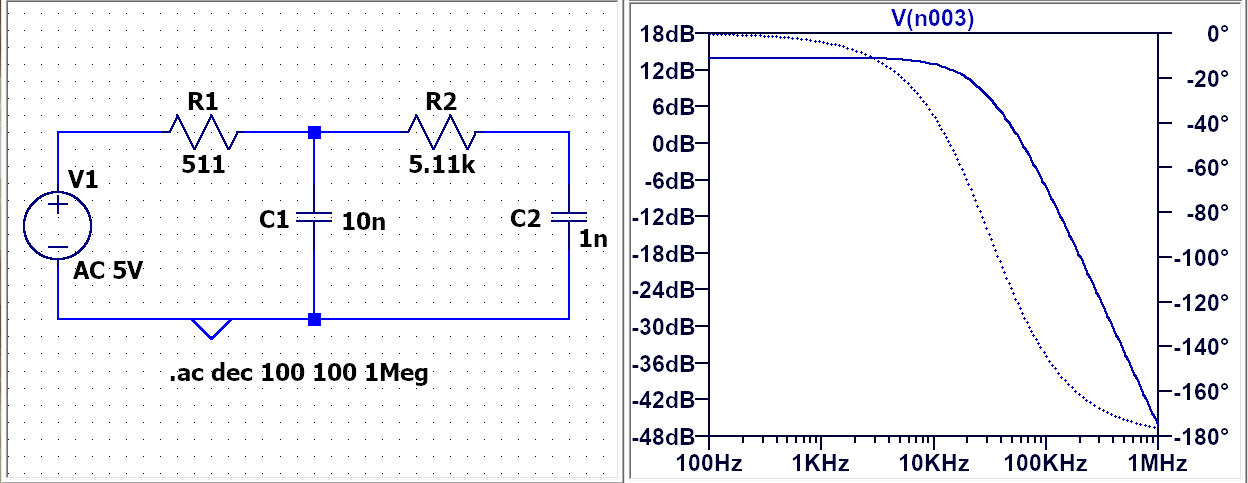
\includegraphics[width=\textwidth]{freq-resp.png}
	}
	-3 dB cutoff frequency = \res{18.672kHz}
\end{figure}


\usubsection{Result}
Designed and simulated a 2 stage RC low pass filter.

It's cutoff frequency was found to be: \res{18.672kHz}

\newpage
\usection{Zener Series Regulator}
\vspace*{1cm}
\linespread{.9}
\usubsection{Aim}
\begin{enumerate}
  \item To design and simulate a zener series voltage regulator for a output voltage of +10V and maximum current of 100mA. (input voltage varies from 12V to 22V)
  \item Plot and its load regulation and line regulation and find percentage load regulation
\end{enumerate}

\usubsection{Design}

\begin{itemize}
  \item $V_Z = 5.1\V$ (\href{https://electronics.stackexchange.com/a/485566/356797}{\underline{using modified BZX84B8V2L with $BV$=5.1V}})
  \item $V_o = 10\V$ \hspace*{.5cm} $V_{in}(max) = 22\V$
  \item $I_D = I_Z(min) = 5\mA$ \hspace*{.5cm} $I_{C2} = 2\mA$
  \item $h_{fe}$ for Q1 (2N3055): $\beta_1 = 15 $\hspace*{.5cm} $h_{fe}$ for Q2 (BC547): $\beta_2$ = 100
\end{itemize}
\begin{align*}
  & V_{RD} = V_o - V_Z = 4.9\V \\[7pt]
  & R_D = \frac{V_{RD}}{I_Z(min)} = \frac{4.9\V}{5\mA} = 980\Omega \\[20pt]
  & \text{\underline{For transistor Q2:}} \\
  & I_{B2} = \frac{I_{C2}}{\beta_2} = 20\mu \text{A} \\[7pt]
  & V_{R2} = V_Z + V_{BE2} = 5.1\V + 0.7\V = 5.8\V \\[7pt]
  & V_{R1} = V_o + V_{R2} = 10\V + 5.8\V = 4.2\V \\[10pt]
  & I_{R1} = 10I_{B2} = 0.2\mA \hspace*{.7cm} I_{R2} = 9I_{B2} = 0.18\mA \\[7pt]
  & R_2 = \frac{V_{R2}}{I_{R2}} = \frac{5.8\V}{0.18\mA} \approx 32\kO\\[10pt]
  & R_1 = \frac{V_{R1}}{I_{R1}} = \frac{4.2\V}{0.2\mA} = 21\kO \\[20pt]
  & \text{\underline{For transistor Q1:}} \\
  & I_{E1} = I_L + I_{R1} + I_{D} = 100\mA + 0.2\mA + 5\mA \approx 105\mA \\[7pt]
  & I_{B1} = \frac{I_{E1}}{\beta_1} = \frac{105\mA}{15} = 7\mA
\end{align*}

\begin{align*}
  & I_{R3} = I_{B1} + I_{C2} = 7\mA + 2\mA = 9\mA\\[7pt]
  & \therefore R_3 = \frac{V_{in}(max) - (V_{BE1} + V_o)}{I_{R3}} \\[10pt]
  & \ \ \ \ \ \ \ = \frac{22\V - (0.7\V + 10\V)}{9\mA} = 1.26\kO
\end{align*}

\usubsection{Circuit, Load \& line regulation}
\uusubsection{Load regulation}
\begin{figure}[H]
  \includegraphics*[width=\textwidth]{load-reg.png}%
\end{figure}

\begin{align*}
  \text{Load Regulation} & = \dfrac{V_{NL} - V_{FL}}{V_{NL}}\times 100\% \\[10pt]
  & = \dfrac{9.9587 - 9.8387}{9.9587}\times 100\% \\[10pt]
  & = \res{1.20\%}
\end{align*}

\vspace*{.5cm}
\uusubsection{Line regulation}
\begin{figure}[H]
  \includegraphics*[width=\textwidth]{line-reg.png}%
\end{figure}
\begin{flalign*}
  \text{Line Regulation} & = \dfrac{\Delta V_{out}}{\Delta V_{in}} \times 100\% \\[10pt]
  & = \dfrac{\Delta V(n002)}{\Delta V(n001)} \times 100\% \\[10pt]
  & = \dfrac{10.2544 - 9.6197}{22 - 12} \times 100\% \\[10pt]
  & = \res{6.35\%}
\end{flalign*}

\usubsection{Result}

Design and simulated a zener series voltage regulator and obtained its regulation parameters:

Load regulation = 6.35\%

Line regulation = 1.20\%

\end{document}
